\section{Mathematical Framework (Implementation)}\label{sec:c6s2}
\kant[8-12]

This section builds on the material in \cref{sec:c6s1}, \cref{ch:7} and the prior work of \citet{ch6-10}; see also \citep{ch6-4,ch6-11}.

\begin{equation}\label{eq:c6s2-a}
  I = \int_{0}^{1}\!\!\int_{0}^{1} \frac{\sin(\pi x)\sin(\pi y)}{1+x^2+y^2}\,\mathrm{d}x\,\mathrm{d}y \approx \frac{1}{M}\sum_{m=1}^{M} h(\xi_m),
\end{equation}
with variance decreasing as
\begin{equation}\label{eq:c6s2-b}
  \operatorname{Var}\bigl[\hat I_M\bigr] = \frac{1}{M}\Bigl(\int h^2\,\mathrm{d}\mu - I^2\Bigr) = \mathcal{O}(M^{-1}).
\end{equation}

Equations~\eqref{eq:c6s2-a} and~\eqref{eq:c6s2-b} are used throughout the remainder of this section.

\lipsum[138-139]

\subsection{Quantitative behaviour}\label{sec:c6s2-q}
Results are collected in \cref{tab:c6s2} and visualised in \cref{fig:c6s2-f1}. Similar trends were reported in~\citep{ch6-5,ch6-7}.

\begin{table}[htbp]
\centering
\caption{Summary of measured quantities for experiment set \texttt{c6s2}.}\label{tab:c6s2}
\begin{tabular}{lrrr}
\toprule
Method & Score & Latency & Error \\
\midrule
Alpha & \num{65.0} & \SI{9.80}{\milli\second} & \num{5.091e-2} \\
Beta & \num{41.0} & \SI{2.49}{\milli\second} & \num{2.640e-5} \\
Gamma & \num{94.6} & \SI{5.42}{\milli\second} & \num{2.299e-3} \\
Delta & \num{55.0} & \SI{0.57}{\milli\second} & \num{1.954e-4} \\
Epsilon & \num{97.6} & \SI{8.67}{\milli\second} & \num{3.459e-5} \\
\bottomrule
\end{tabular}
\end{table}

\begin{figure}[htbp]
\centering
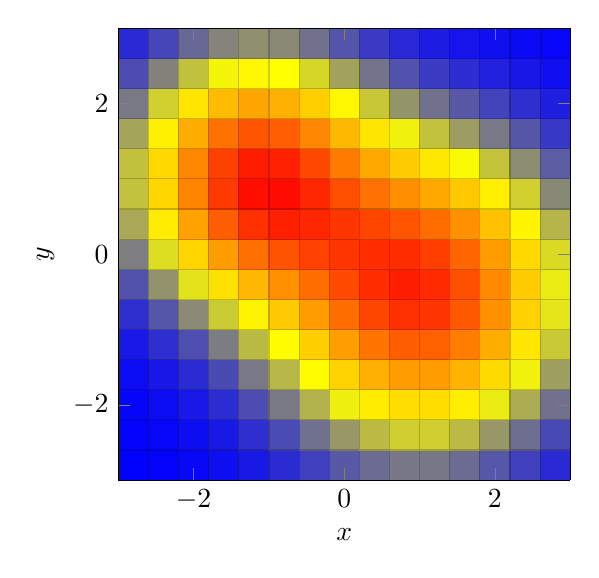
\begin{tikzpicture}\begin{axis}[width=0.7\linewidth,view={0}{90},colormap/hot,xlabel=$x$,ylabel=$y$,axis equal image]
\addplot3[surf,samples=16,domain=-3:3]{exp(-((x-1)^2+(y+0.5)^2)/3.0)+exp(-((x+1.2)^2+(y-1)^2)/2.0)};
\end{axis}\end{tikzpicture}
\caption{Generated figure for \texttt{c6s2-f1} (parameters $a=5$, $b=6$).}\label{fig:c6s2-f1}
\end{figure}

\lipsum[45-46]

\subsection{Implementation notes}\label{sec:c6s2-i}
The core routine is shown in \cref{lst:c6s2}; its complexity is $\mathcal{O}(N\log N)$ per iteration~\cite{ch6-3}.

\begin{lstlisting}[language=python,caption={Reference implementation for c6s2.},label={lst:c6s2}]
def conjugate_gradient(A, b, tol=1e-8, maxit=500):
    x = b * 0
    r = b - A @ x
    p = r.copy()
    for k in range(maxit):
        Ap = A @ p
        alpha = (r @ r) / (p @ Ap)
        x += alpha * p
        r_new = r - alpha * Ap
        if (r_new @ r_new) ** 0.5 < tol:
            break
        p = r_new + ((r_new @ r_new) / (r @ r)) * p
        r = r_new
    return x
\end{lstlisting}

\lipsum[115-115]
\begin{theorem}\label{thm:c6s2}
Let $A\in\mathbb{R}^{n\times n}$ be symmetric positive definite with condition number $\kappa$. Then the iteration converges and
$\lVert e_k\rVert_A \le 2\bigl(\tfrac{\sqrt\kappa-1}{\sqrt\kappa+1}\bigr)^k\lVert e_0\rVert_A$.
\end{theorem}
\begin{enumerate}[label=(\roman*)]
\item the bound in \cref{thm:c6s2} is sharp for some initial errors;
\item the constant $2$ cannot be improved in general;
\item preconditioning reduces the effective $\kappa$.
\end{enumerate}

\begin{figure}[htbp]
\centering
\includegraphics[width=0.45\linewidth]{schematic.pdf}
\caption{Raster/vector asset \texttt{schematic.pdf} included from the figures directory.}\label{fig:c6s2-i0}
\end{figure}

\begin{figure}[htbp]
\centering
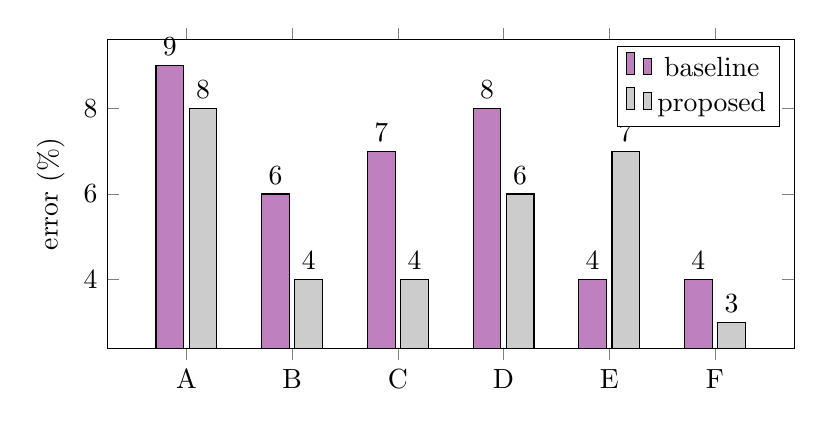
\begin{tikzpicture}\begin{axis}[ybar,width=0.85\linewidth,height=5.5cm,symbolic x coords={A,B,C,D,E,F},xtick=data,ylabel={error (\%)},enlarge x limits=0.15,bar width=10pt,nodes near coords]
\addplot[fill=violet!50] coordinates {(A,9) (B,6) (C,7) (D,8) (E,4) (F,4)};
\addplot[fill=gray!40] coordinates {(A,8) (B,4) (C,4) (D,6) (E,7) (F,3)};
\legend{baseline,proposed}
\end{axis}\end{tikzpicture}
\caption{Generated figure for \texttt{c6s2-f2} (parameters $a=3$, $b=4$).}\label{fig:c6s2-f2}
\end{figure}

\lipsum[107-107]
